\documentclass[11pt,a4paper]{article}
\usepackage[T1]{fontenc}
\usepackage[utf8]{inputenc}
\usepackage{lmodern}
\usepackage{amsmath,amssymb,amsthm,mathtools,mathrsfs}
\usepackage{graphicx,float,xcolor,multicol}
\usepackage[shortlabels]{enumitem}
\usepackage[margin=27mm]{geometry}
\usepackage{microtype,needspace,placeins}
\usepackage{tikz,tikz-cd}
\usetikzlibrary{arrows.meta,calc,positioning,patterns,decorations.pathreplacing}
\usepackage[colorlinks=true,linkcolor=teal,urlcolor=teal,citecolor=teal]{hyperref}
\setlength{\parindent}{0pt}
\setlength{\parskip}{.6em}
\setcounter{secnumdepth}{0}
\allowdisplaybreaks
\raggedbottom
\providecommand{\cross}{\times}
\DeclareUnicodeCharacter{2020}{\ensuremath{\dagger}}
\DeclareMathOperator{\supp}{supp}
\DeclareMathOperator*{\esssup}{ess\,sup}
\providecommand{\chapter}{\section}
\newenvironment{tool}[2]{\subsection*{Tool #1 --- #2}}{}
\newcommand{\ToolRef}[1]{Tool #1}
\newcommand{\FigureTag}[2]{\textit{Figure #1}}
\newcommand{\Result}[1]{\subsection*{#1}}
\newcommand{\Application}[1]{\subsubsection*{Application\if\relax\detokenize{#1}\relax\else\space--- #1\fi}}
\newcommand{\ProofHeading}{\par\textit{Proof.}\space}
\newcommand{\ProofOf}[1]{\par\textit{Proof of #1.}\space}
\newcommand{\RemarkHeading}{\par\textbf{Remark.}\space}
\newcommand{\NoteHeading}{\par\textbf{Note.}\space}
\newcommand{\ExerciseHeading}{\par\textbf{Exercise.}\space}

\graphicspath{{figures/complex-analysis/}}
\begin{document}
\section*{Liouville and Morera}
% BLOG-CONTENT-BEGIN
\subsection*{Tool 14 — Schwarz Lemma}

Let \(f\colon B_1(0)\to B_1(0)\)
be holomorphic, with $f(0)=0$. Then:
\begin{enumerate}
  \item[(i)] $|f(z)|\leq |z|$ for every $z\in B_1(0)$;
  \item[(ii)] if $|f(z_0)|=|z_0|$ for some $z_0$, then $f$ is a rotation;
  \item[(iii)] $|f'(0)|\leq1$, and if equality holds, then $f$ is a rotation.
\end{enumerate}


\textit{Proof.}
We have
\[
  f(z)=z\left(\sum_{n\geq0}a_n z^n\right),
\]
and hence
\[
  \frac{f(z)}{z}\in H(B_1(0)).
\]
Now, for $|z|=r<1$, \(\left|\frac{f(z)}{z}\right|\leq\frac1r.\)
Therefore
\[
  \left|\frac{f(z)}{z}\right|
  \leq\inf_r\frac1r=1,
\]
and thus
\[
  \left|\frac{f(z)}{z}\right|\leq1
  \quad\Longrightarrow\quad
  |f(z)|\leq|z|.
\]
If $|f(z_0)|=|z_0|$, then


$f(z)/z$ attains a maximum in the interior, so $f(z)=cz$. But, as
$|f(z_0)|=|z_0|$, we have $|c|=1$. Therefore $f$ is a rotation.

Let
\[
  \frac{f(z)}{z}=g(z),
  \qquad g\in H(B_1(0)).
\]
Then
\[
  g(0)=\lim_{z\to0}\frac{f(z)}{z}
      =\lim_{z\to0}\frac{f(z)-f(0)}{z}
      =f'(0).
\]
Since $|g(z)|\leq1$, \(|g(0)|=|f'(0)|\leq1.\)
If equality holds, then $g(0)=1$, so $g$ is a constant and $f/z$ is a
constant. Hence
\[
  f=cz,
  \qquad f'(0)=1,
  \qquad |c|=1.
\]

\subsection*{Tool 15 — Morera's Theorem}
(We saw a proof of this recently.)


\subsection*{Tool 16 — Liouville's Theorem}
An entire bounded function is constant.


\subsubsection*{Application — Liouville and Morera}
Let us see two instances of each.

\subsection*{Fundamental Theorem of Algebra}

\textit{Proof.}
Let $p(z)$ be a polynomial. Since $|p(z)|\to\infty$ as $|z|\to\infty$, we
have $1/p(z)$ bounded and entire if $p$ never vanishes. Hence $p$ is a
constant, a contradiction.

\subsection*{Casorati--Weierstrass}
Let
\[
  f\in H\bigl(B_r(z_0)\setminus\{z_0\}\bigr),
\]
and suppose that $f$ has an essential singularity at $z_0$. Then
\[
  f\bigl(B_r(z_0)\setminus\{z_0\}\bigr)
\]
is dense in $\mathbb C$.


\textit{Proof.}
Suppose there exists $w\in\mathbb C$ such that
$f(B_r(z_0)\setminus\{z_0\})$ stays away from it. Then there exists
$\delta>0$ such that
\[
  |f(z)-w|>\delta
  \qquad\forall z\in B_r(z_0)\setminus\{z_0\}.
\]
Thus \(|g(z)|=\left|\frac1{f(z)-w}\right|<\frac1\delta,\)
so $g$ has a removable singularity at $z_0$. Hence $f-w$ either has a
removable singularity at $z_0$ or a pole at $z_0$, depending on whether
$g(z_0)\neq0$ or $g(z_0)=0$.

\subsection*{Tool 17 — Weierstrass Convergence Theorem}
Let $\{f_n\}_n$ be such that $f_n\in H(\Omega)$ and $f_n\to f$ uniformly on
compact sets. Then $f\in H(\Omega)$.


\textbf{Note.}
This result is intended to be shown as an instance of Morera's Theorem, but it
turns out to be a technique in itself. So we prove it to serve our purpose.

\textit{Proof.}
Let $D$ be a disc in $\Omega$, and let $\gamma$ be a polygonal path in $D$.
We know
\[
  \int_\gamma f_n\,dz=0.
\]
As $f_n\to f$ uniformly in $\overline D$,
\[
  \int_\gamma f_n\to\int_\gamma f,
\]
so $\int_\gamma f=0$. Also, $f$ is continuous, and hence $f\in H(D)$. This is
true for all $D$ in $\Omega$, so $f\in H(\Omega)$.

Let us see two instances of Tool 17 before we show another instance of Morera
in action.

\subsubsection*{Application — Convergence of derivatives}
Under the hypotheses of Tool 17, \(f_n'\to f'\)
uniformly on all compact sets of $\Omega$.

\textit{Proof.}
Set
\[
  \Omega_\delta
  :=\bigl\{z\in\Omega\mid \overline{D_\delta(z)}\subset\Omega\bigr\}.
\]


Given any compact set, there exists $r$ such that $B_r(z)$, for $z$ in that
compact set, is in $\Omega$. Thus that compact set is contained in
$\Omega_\delta$ for some $\delta$. Therefore it suffices to show the result on
$\Omega_\delta$. Set $F=f_n-f$. We have
\[
  F'(z)=\frac1{2\pi i}\int_{C_\delta(z)}\frac{F(t)}{(t-z)^2}\,dt,
\]
where $C_\delta(z)$ is the circle of radius $\delta$, for $z\in\Omega_\delta$.
Therefore
\[
  |F'(z)|
  \leq\frac1{2\pi}\sup_{t\in C_\delta(z)}|F(t)|\frac1{\delta^2}(2\pi\delta)
  \leq\frac1\delta\sup_{t\in\Omega}|F(t)|,
\]
and hence
\[
  \sup_{z\in\Omega_\delta}|F'(z)|
  \leq\frac1\delta\sup_{t\in\Omega}|F(t)|.
\]
Thus $f_n'\to f'$ uniformly on all compact sets.

\subsubsection*{Application — Holomorphic parameter integrals}
Let $F$ be continuous on $\Omega\times[0,1]$, and
suppose that, for every $s\in[0,1]$, $F(z,s)\in H(\Omega)$. Let
\[
  f(z)=\int_0^1F(z,s)\,ds.
\]
Then $f\in H(\Omega)$.

\textit{Proof.}
Define
\[
  f_n(z):=\frac1n\sum_{k=1}^n F\left(z,\frac kn\right).
\]
Then $f_n$ is holomorphic. The function $F$ is uniformly continuous on
$D\times[0,1]$, a cylinder. Thus, for every $\varepsilon$, there exists
$\delta$ such that
\[
  |F(z,s_1)-F(z,s_2)|<\varepsilon
  \quad\text{if }|s_1-s_2|<\delta,
  \qquad\forall z\in D.
\]
Set $1/n<\delta$. Then
\begin{align*}
  |f_n(z)-f(z)|
  &=\left|
    \sum_{k=1}^n\int_{(k-1)/n}^{k/n}
    \left(F\left(z,\frac kn\right)-F(z,s)\right)ds
  \right|\\
  &\leq\sum_{k=1}^n\int_{(k-1)/n}^{k/n}
    \left|F\left(z,\frac kn\right)-F(z,s)\right|ds\\
  &<\sum_{k=1}^n\frac\varepsilon n
  <\varepsilon.
\end{align*}
Thus, on $\overline D$, $f_n\to f$ uniformly, and hence $f\in H(\Omega)$.

\textbf{Remark.}
Using these two results, one can construct elements in $H(\Omega)$ such as
$\sum_{n\geq0}f_n(z)$.


\subsection*{Tool 18 — Schwarz Reflection Principle}
Let $U$ be a domain in $\mathbb C$ such that \(\bar z\in U\iff z\in U.\)
Let
\[
  f_+\in H\bigl(\{z\in U\mid\operatorname{Im}(z)>0\}\bigr),
  \qquad
  f_-\in H\bigl(\{z\in U\mid\operatorname{Im}(z)<0\}\bigr).
\]
Suppose $f_+$ and $f_-$ extend continuously to
$\{z\in U\mid\operatorname{Im}(z)=0\}$ and agree there. Then $f_+$ and $f_-$
are restrictions of a single holomorphic function $f\in H(U)$.


\textit{Proof.}
By the pasting lemma, we see that $f$ is continuous on $U$. Let $T$ be a
triangle in $U$.

\begin{figure}[htbp]
  \centering
  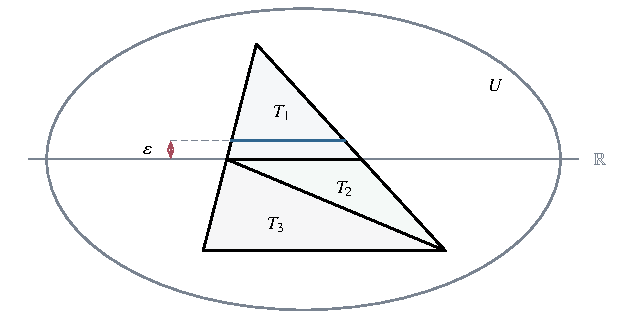
\includegraphics[width=.66\textwidth]{note4-fig-01.pdf}

\end{figure}
\emph{Annotation:} ``Pardon the asymmetry!''

Set
\[
  f=
  \begin{cases}
    f^+,&\text{on }U^+,\\
    f^+=f^-,&\text{on }U\cap\mathbb R,\\
    f^-,&\text{on }U^-.
  \end{cases}
\]
Then
\[
  \int_{T_i}f(z)\,dz=0,
  \qquad i=1,2,3.
\]
As $\varepsilon\to0$, we see that
\[
  \int_T f(z)\,dz=0.
\]
Morera gives the result. The only apparently clear subtlety is in seeing that
the integrals of these triangles vary continuously as $\varepsilon\to0$; that
is seen once one writes the parametrizations.


\textbf{Remark.}
In this way, a function $f\in H(U^+)$ that extends continuously to
$\overline{U^+}$ can be extended to $U$ once we set
\[
  f(z)=\overline{f(\bar z)}
  \qquad\text{on }U^-.
\]

Here is an interesting instance of the Schwarz Reflection Principle.

\subsubsection*{Application}
Suppose $f(z)\neq0$ is continuous on $\overline D$ and
$f\in H(D)$, and \(|f(z)|=1\iff |z|=1.\)
Then $f$ is a constant.

\textit{Proof.}
If one can mimic Schwarz's proof here with the extension
\[
  f(z)=\frac1{\overline{f(1/\bar z)}}
  \qquad(\forall z, |z|>1),
\]
then we are done. Continuity of $f$ is ensured by the pasting lemma. We just
have to make sure that its integral on triangles vanishes. As before, set
\[
  f=
  \begin{cases}
    f(z),&\forall z\in\overline D,\\[2mm]
    \displaystyle\frac1{\overline{f(1/\bar z)}},&\forall z\in D^c.
  \end{cases}
\]
We shall exploit the convexity of $D$. Let $T$ be a triangle in $\mathbb C$.

\begin{figure}[htbp]
  \centering
  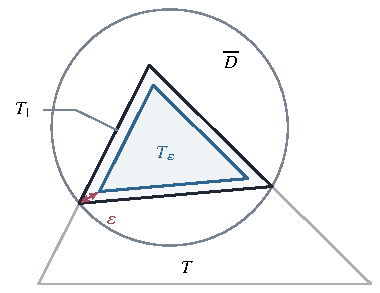
\includegraphics[width=.48\textwidth]{note4-fig-02.pdf}

\end{figure}

Push $T_\varepsilon\to T_1$ so that we have
\[
  \int_{T_\varepsilon}f(z)\,dz
  =\int_{T_1}f(z)\,dz
  =0.
\]
Now let us construct polygons.


\begin{figure}[htbp]
  \centering
  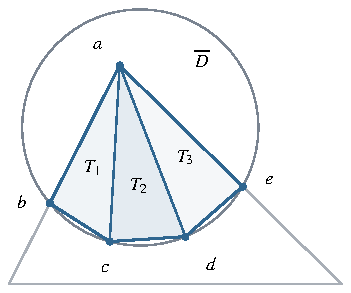
\includegraphics[width=.44\textwidth]{note4-fig-03.pdf}

\end{figure}

By pushing down as before, we see that
\[
  \int_{T_1}f(z)\,dz
  =\int_{T_2}f(z)\,dz
  =\int_{T_3}f(z)\,dz
  =0.
\]
Therefore
\[
  \int_{\gamma_{a\to b\to c\to d\to e\to a}}f(z)\,dz
  =\sum_{i=1}^{2}\int_{T_i}f(z)\,dz
  =0.
\]

Now approximate the arc with polygons to finally get
\[
  \int_\gamma f(z)\,dz=0.
\]
Similarly, one can prove
\[
  \int_{\gamma'}f(z)\,dz=0.
\]

\begin{figure}[htbp]
  \centering
  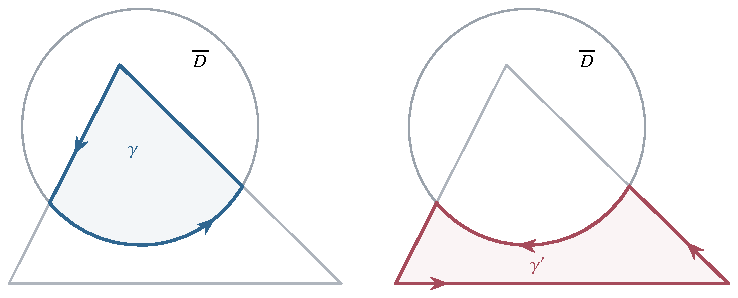
\includegraphics[width=.90\textwidth]{note4-fig-04.pdf}

\end{figure}

Hence
\[
  \int_T f(z)\,dz=0,
\]
so $f\in H(\mathbb C)$. But $f$ is bounded, and therefore $f$ is constant.

\textbf{Exercise.}
Make this geometric argument analytic. Do it!


The following is not a standard technique, but it is a useful tool to have in
one's arsenal.

\subsection*{Tool 19 — Reverse Triangle Inequality}
Given $\{z_i\}_{i=1}^N$, with $z_i\in\mathbb C$, there exists
$S\subseteq\{1,2,\ldots,N\}$ such that
\[
  \left|\sum_{k\in S}z_k\right|
  \geq\frac1\pi\sum_{k=1}^N|z_k|.
\]
(Reverse Triangle Inequality.)


\textit{Proof.}
Set \(z_k=|z_k|e^{i\alpha_k}.\)
For $-\pi\leq\theta\leq\pi$, let $S(\theta)$ be the set of all $k$ such that
\[
  \cos(\alpha_k-\theta)>0.
\]
Then

\[
  \left|\sum_{S(\theta)}z_k\right|
  =\left|\sum_{S(\theta)}e^{-i\theta}z_k\right|
  \geq\operatorname{Re}\sum_{S(\theta)}e^{-i\theta}z_k
  =\sum_{k=1}^N|z_k|\cos^+(\alpha_k-\theta),
\]
where
\[
  \cos^+\theta:=\max(\cos\theta,0).
\]
Let $\theta_0$ be such that the last sum is maximum in $[-\pi,\pi]$, and let
$S=S(\theta_0)$. Then
\begin{align*}
  \left|\sum_S z_k\right|
  &\geq\sum_{k=1}^N|z_k|\cos^+(\alpha_k-\theta_0)\\
  &=\sup_\theta\left(
    \sum_{k=1}^N|z_k|\cos^+(\alpha_k-\theta)
  \right).
\end{align*}
Now put
\[
  M_\theta:=\sum_{k=1}^N|z_k|\cos^+(\alpha_k-\theta).
\]
Then
\[
  2\pi\sup_\theta M_\theta
  \approx
  \sum_{i=1}^N M_{\theta_i}\left(\frac{N}{2\pi}\right)^{-1};
\]
that is,
\[
  \sup_\theta M_\theta
  \geq\frac1{2\pi}\int_{-\pi}^{\pi}M_\theta\,d\theta.
\]
Consequently,
\begin{align*}
  \sup_\theta M_\theta
  &\geq\frac1{2\pi}\sum_{k=1}^N|z_k|
    \int_{-\pi}^{\pi}\cos^+(\alpha_k-\theta)\,d\theta\\
  &=\frac1\pi\sum_{k=1}^N|z_k|.
\end{align*}
% BLOG-CONTENT-END
\end{document}
